\usetikzlibrary{positioning, shapes.geometric, arrows.meta, fit, backgrounds, calc}


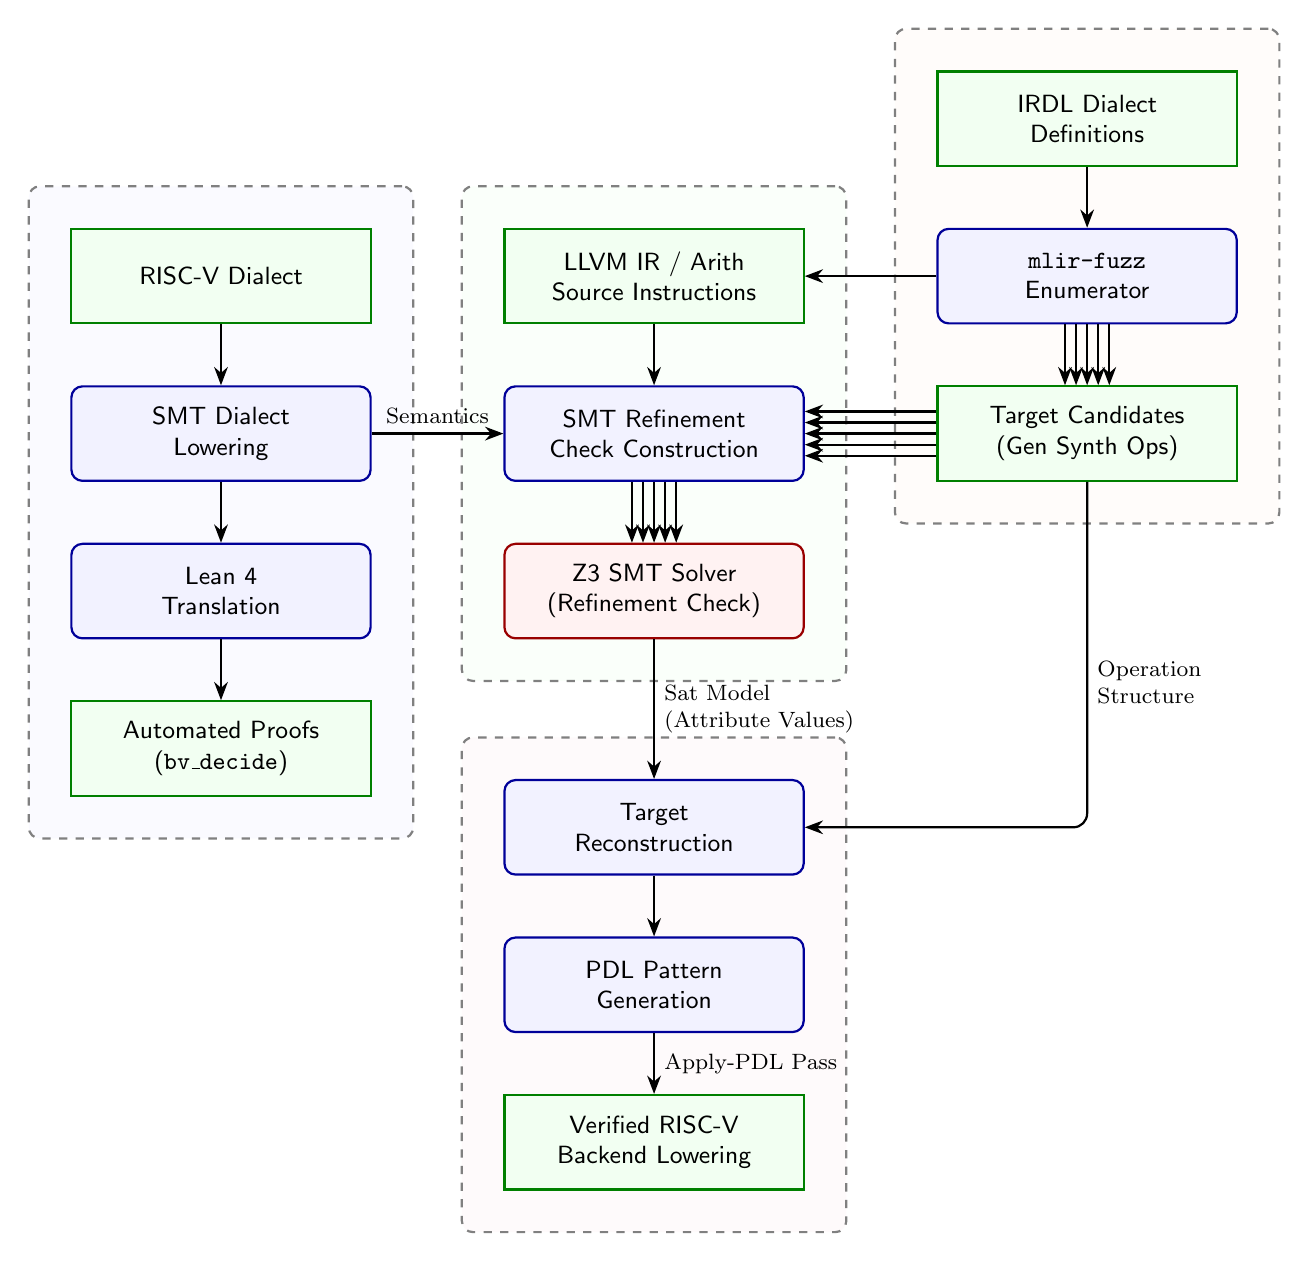
\begin{tikzpicture}[
    >=Stealth,
    process/.style={rectangle, rounded corners, draw=blue!60!black, fill=blue!5, thick, minimum width=3.8cm, minimum height=1.2cm, align=center, text width=3.4cm, font=\small\sffamily},
    artifact/.style={rectangle, draw=green!50!black, fill=green!5, thick, minimum width=3.8cm, minimum height=1.2cm, align=center, text width=3.4cm, font=\small\sffamily},
    solver/.style={rectangle, rounded corners, draw=red!60!black, fill=red!5, thick, minimum width=3.8cm, minimum height=1.2cm, align=center, text width=3.4cm, font=\small\sffamily},
    groupbox/.style={rectangle, draw=gray, dashed, thick, inner sep=15pt, rounded corners},
    grouptitle/.style={font=\sffamily\bfseries, text=gray!80!black, fill=white, inner sep=2pt}
]

    \node[artifact] at (0, 2) (source) {LLVM IR / Arith \\ Source Instructions};
    \node[process]  at (0, 0) (formulation) {SMT Refinement \\ Check Construction};
    \node[solver]   at (0, -2) (z3) {Z3 SMT Solver \\ (Refinement Check)};

    \node[artifact] at (-5.5, 2) (riscv) {RISC-V Dialect};
    \node[process]  at (-5.5, 0) (smtlow) {SMT Dialect \\ Lowering};
    \node[process]  at (-5.5, -2) (lean) {Lean 4 \\ Translation};
    \node[artifact] at (-5.5, -4) (proof) {Automated Proofs \\ (\texttt{bv\_decide})};

    \node[artifact] at (5.5, 4) (irdl) {IRDL Dialect \\ Definitions};
    \node[process]  at (5.5, 2) (fuzz) {\texttt{mlir-fuzz} \\ Enumerator};
    \node[artifact] at (5.5, 0) (synth) {Target Candidates \\ (Gen Synth Ops)};

    \node[process]  at (0, -5) (recon) {Target \\ Reconstruction};
    \node[process]  at (0, -7) (pdl) {PDL Pattern \\ Generation};
    \node[artifact] at (0, -9) (backend) {Verified RISC-V \\ Backend Lowering};

    \draw[->, thick] (fuzz) -- (source);

    \draw[->, thick] (riscv) -- (smtlow);
    \draw[->, thick] (smtlow) -- (lean);
    \draw[->, thick] (lean) -- (proof);

    \draw[->, thick] (irdl) -- (fuzz);

		\draw[->, thick] ([xshift=-8pt]fuzz.south) -- ([xshift=-8pt]synth.north);
		\draw[->, thick] ([xshift=-4pt]fuzz.south) -- ([xshift=-4pt]synth.north);
		\draw[->, thick] (fuzz.south) -- (synth.north);
		\draw[->, thick] ([xshift=4pt]fuzz.south) -- ([xshift=4pt]synth.north);
		\draw[->, thick] ([xshift=8pt]fuzz.south) -- ([xshift=8pt]synth.north);

    \draw[->, thick] (smtlow) -- (formulation) node[midway, above, font=\footnotesize] {Semantics};
		\draw[->, thick] ([yshift=8pt]synth.west) -- ([yshift=8pt]formulation.east);
		\draw[->, thick] ([yshift=4pt]synth.west) -- ([yshift=4pt]formulation.east);
		\draw[->, thick] (synth.west) -- (formulation.east);
		\draw[->, thick] ([yshift=-4pt]synth.west) -- ([yshift=-4pt]formulation.east);
		\draw[->, thick] ([yshift=-8pt]synth.west) -- ([yshift=-8pt]formulation.east);

    \draw[->, thick] (source) -- (formulation);
		\draw[->, thick] ([xshift=-8pt]formulation.south) -- ([xshift=-8pt]z3.north);
		\draw[->, thick] ([xshift=-4pt]formulation.south) -- ([xshift=-4pt]z3.north);
		\draw[->, thick] (formulation.south) -- (z3.north);
		\draw[->, thick] ([xshift=4pt]formulation.south) -- ([xshift=4pt]z3.north);
		\draw[->, thick] ([xshift=8pt]formulation.south) -- ([xshift=8pt]z3.north);

    \draw[->, thick] (z3) -- (recon) node[midway, right, align=left, font=\footnotesize] {Sat Model \\ (Attribute Values)};
    \draw[->, thick, rounded corners=5pt] (synth.south) |- (recon.east) node[near start, right, align=left, font=\footnotesize, yshift=-10pt] {Operation \\ Structure};

    \draw[->, thick] (recon) -- (pdl);
    \draw[->, thick] (pdl) -- (backend) node[midway, right, font=\footnotesize] {Apply-PDL Pass};

    \begin{scope}[on background layer]
        \node[groupbox, fill=blue!2, fit=(riscv) (smtlow) (lean) (proof)] (group_sem) {};
        \node[groupbox, fill=orange!2, fit=(irdl) (fuzz) (synth)] (group_enum) {};
        \node[groupbox, fill=green!2, fit=(source) (formulation) (z3)] (group_synth) {};
        \node[groupbox, fill=purple!2, fit=(recon) (pdl) (backend)] (group_recon) {};
    \end{scope}
\end{tikzpicture}